\chapter{Modellierung des Wahlinformationssystems}

Das ER Modell \ref{fig:ER-Diagramm-wahlsystem} stellt die verwendeten Klassen der Datenbank f�r das Wahlinformationssystem dar. Die Klassen enthalten die zun�chst zur Verf�gung stehenden Daten ohne Vorberechnungen. Aus diesen Daten werden �ber mehrere Zwischenschritte die Ausgabedaten ermittelt. Die Zwischenschritte werden in eigenen Tabellen abgespeichert. Je nach Konfiguration k�nnen diese Tabellen tempor�re Tabellen, tempor�re Tabellen innerhalb eines SQL Befehls (``with''), materialisierte Anfragen (Materialized Query Tables) oder normale persistente Tabellen sein. Diese Zwischentabellen sind in Abbildung \ref{fig:Temporaere_Tabellen} dargestellt. Die gr�nen Boxen stellen die Grundklassen dar, wie sie auch im ER Modell \ref{fig:ER-Diagramm-wahlsystem} enthalten sind. Pfeile stellen Berechnungsbeziehungen da. Der Pfeil von ``ErststimmenNachWahlkreis'' nach ``Direktmandate'' bedeutet zum Beispiel, dass die Direktmandate aus den ErststimmenNachWahlkreis durch Aggregation berechnet werden. Die Linien mit Beschriftung ``references'' stellen eine Fremdschl�sselbeziehung dar. Dementsprechend bedeutet die Verbindung zwischen ``Kandidat'' und ``Direktmandate'', dass die Tabelle ``Direktmandate'' ein Attribut enth�lt, dass die ID von ``Kandidat'' referenziert.

\begin{figure}[htbp]
	\centering
		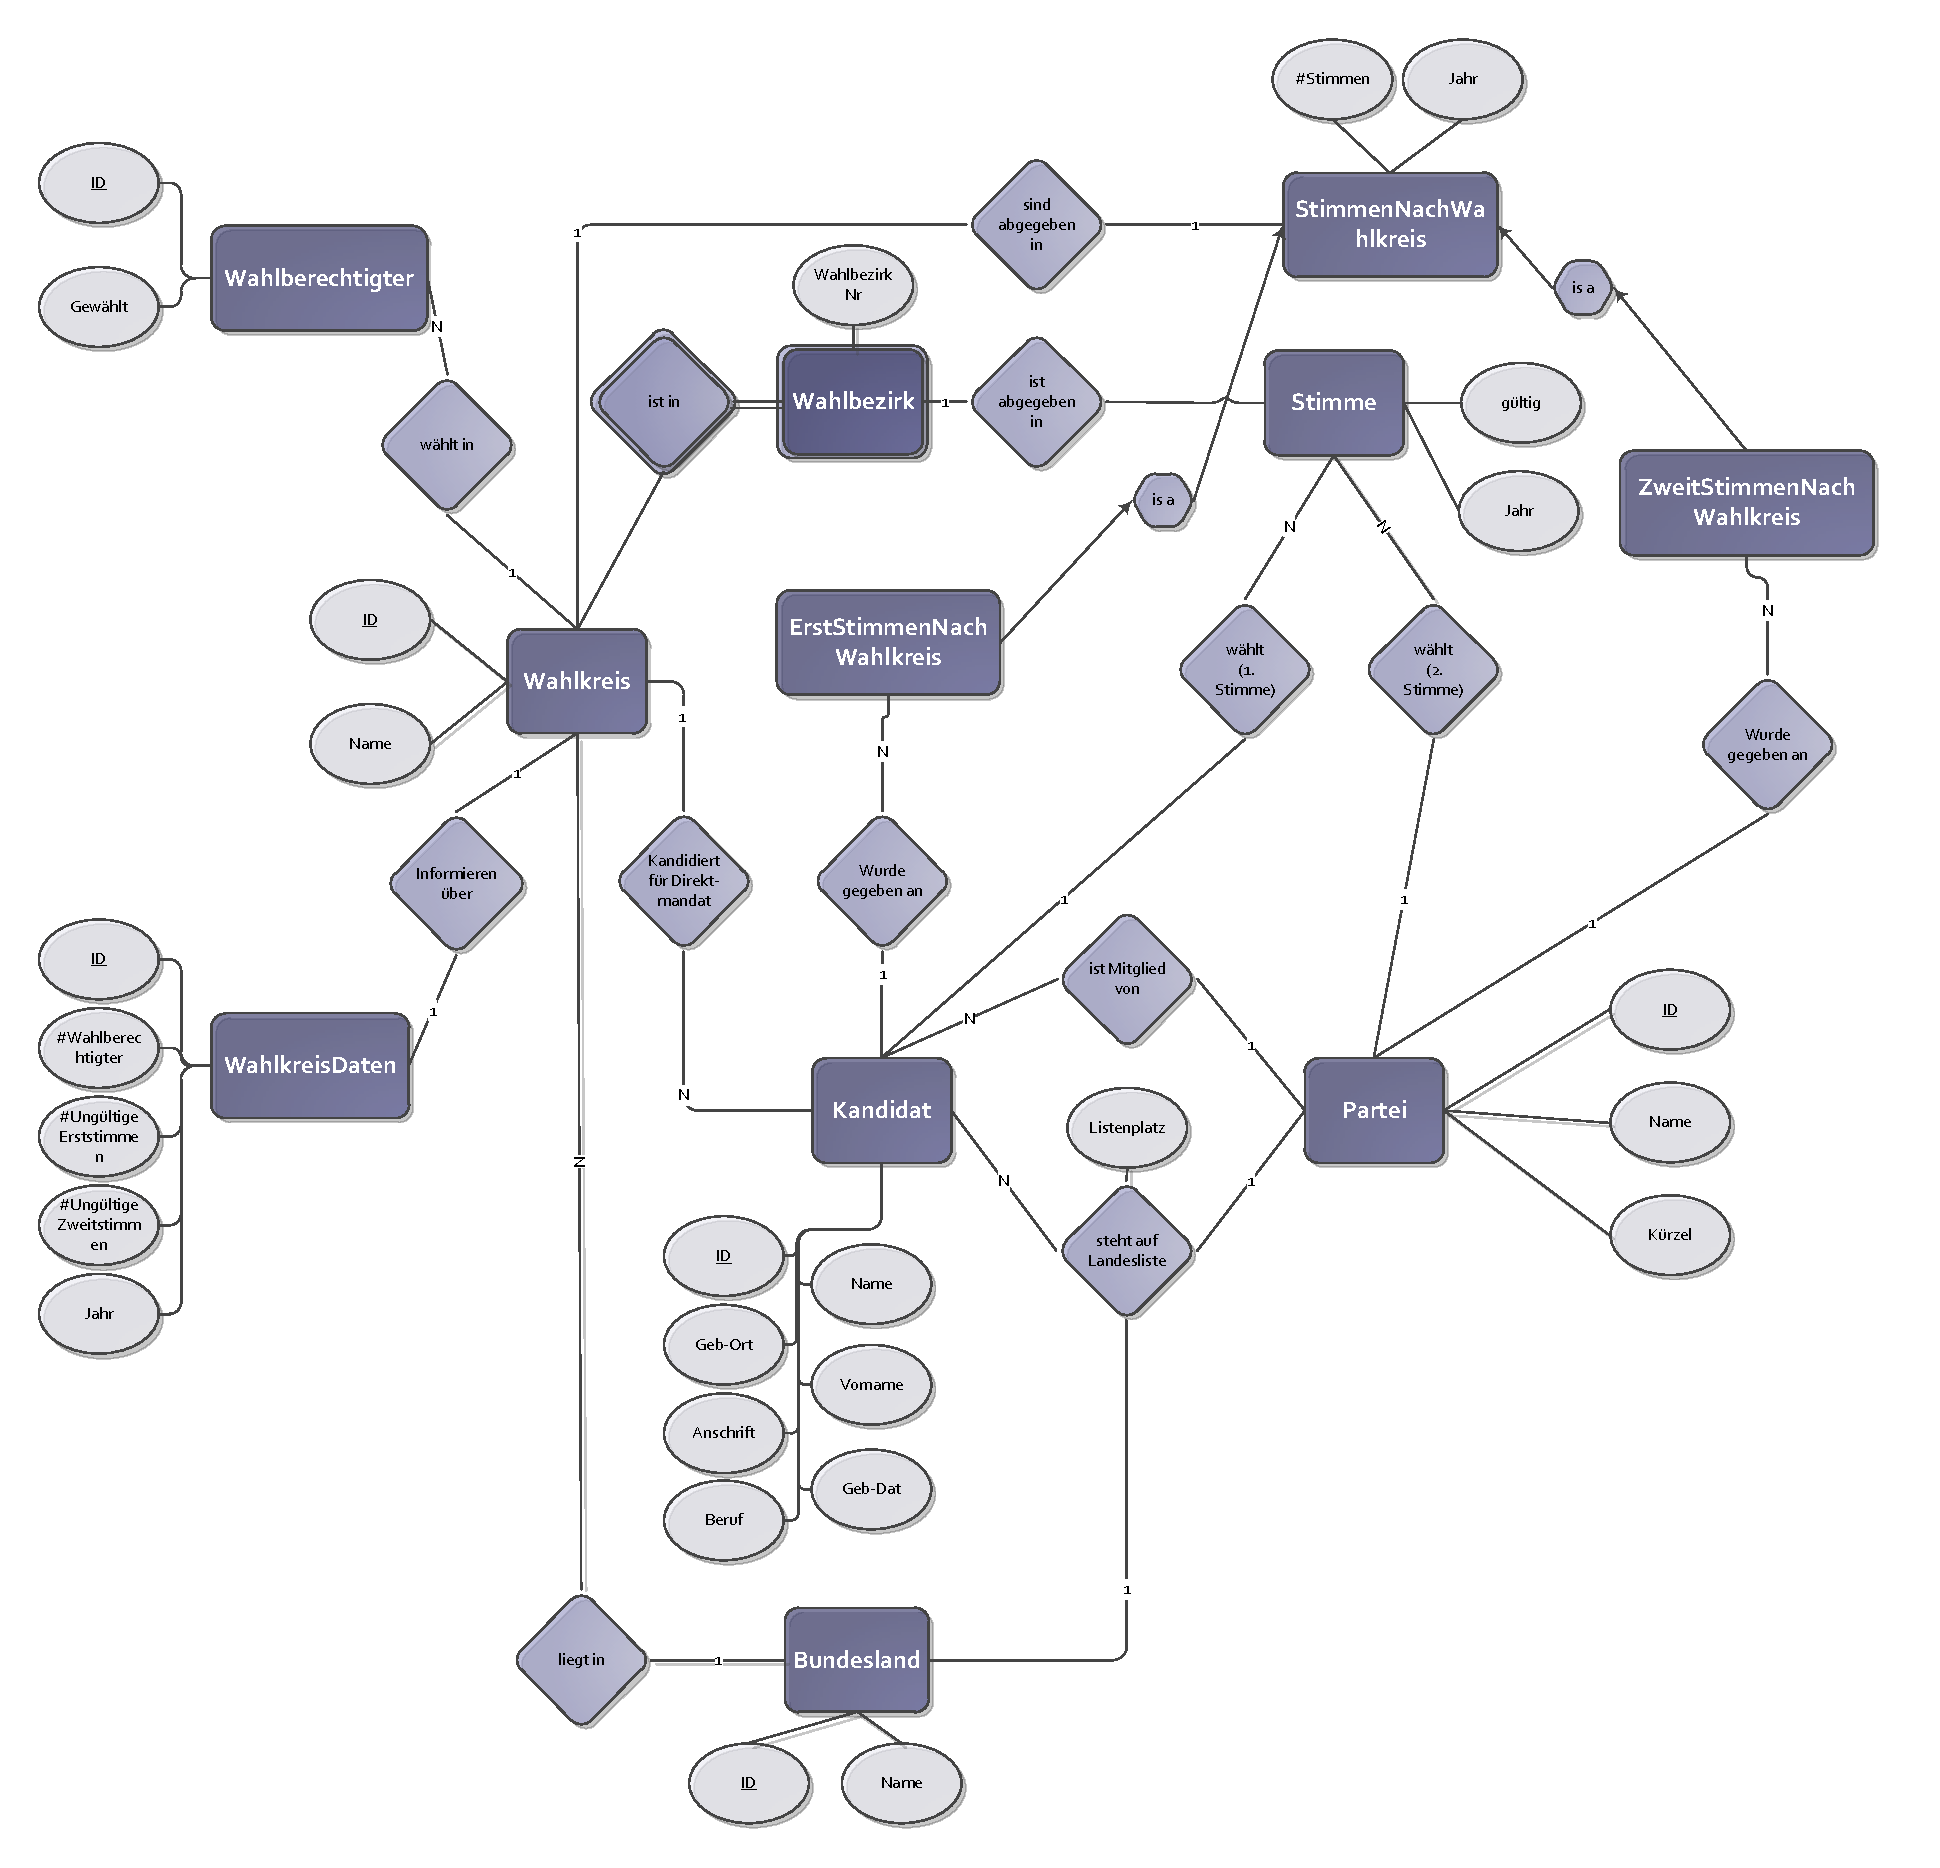
\includegraphics[width=1.00\textwidth]{figures/ER-Diagramm-wahlsystem.pdf}
	\caption{ER Modell des Wahlinformationssystems}
	\label{fig:ER-Diagramm-wahlsystem}
\end{figure}

\begin{figure}[htbp]
	\centering
		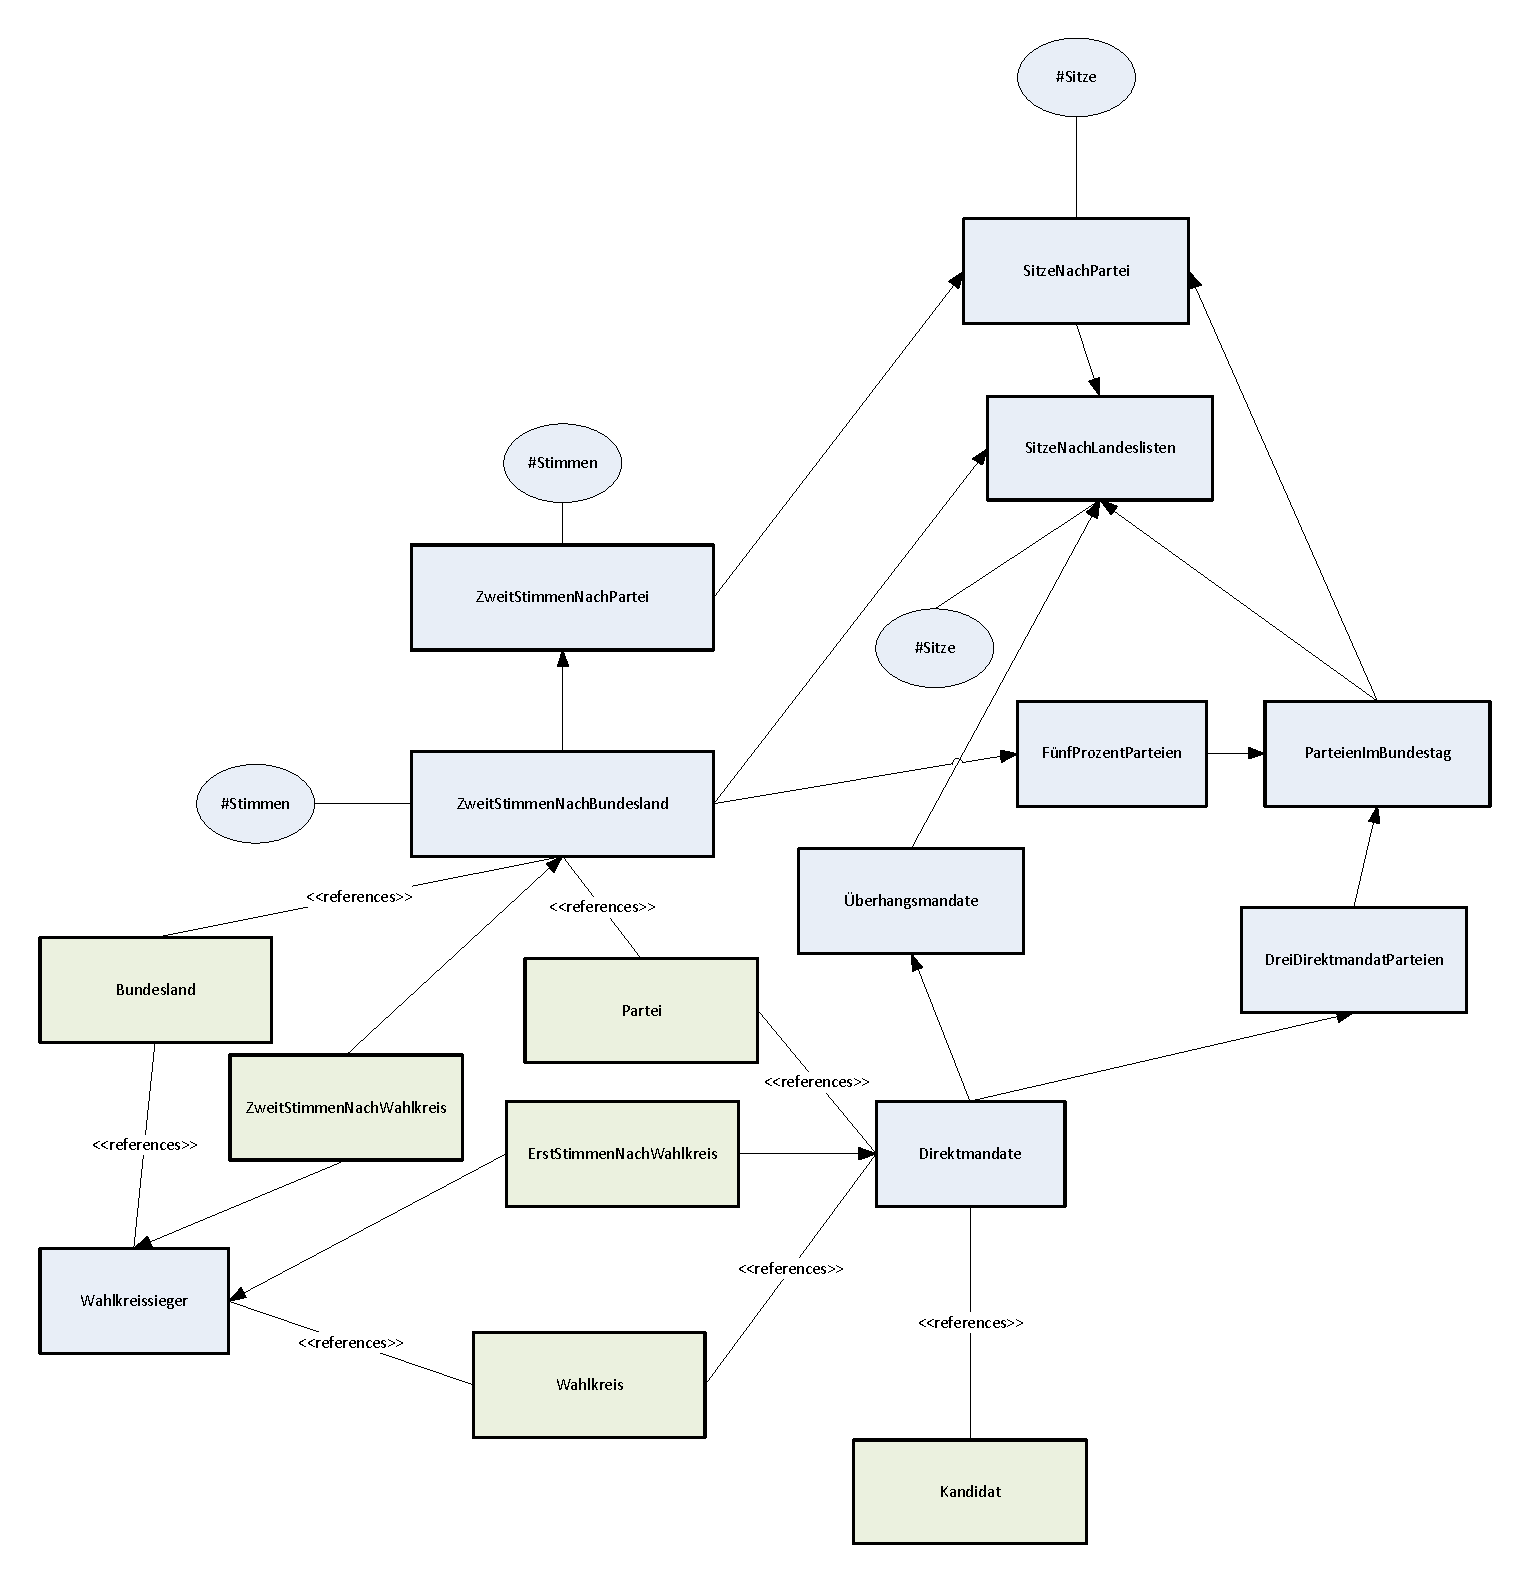
\includegraphics[width=1.00\textwidth]{figures/Temporaere_Tabellen.pdf}
	\caption{Zusammenhang zwischen den Grundtabellen und den tempor�ren Tabellen}
	\label{fig:Temporaere_Tabellen}
\end{figure}

